%!TEX root = ../39.tex

\documentclass[12pt,a4paper]{article}
\pagestyle{plain} \setlength{\textheight}{21cm}
\setlength{\textwidth}{15cm} \setlength{\footskip}{1.0cm}

%\usepackage{harvard}
\usepackage{theorem}
\usepackage{amsmath,amssymb,amsopn}
\usepackage{graphicx,lineno}
\usepackage{verbatim}
\usepackage{lscape}
\usepackage{natbib}
\usepackage{setspace}
\usepackage{rotating}
\usepackage{psfrag}
%\usepackage{booktabs}
\usepackage{enumerate}
\usepackage{url}
%\usepackage[bottomafter,first]{draftcopy}

\newcommand{\rem}[1]{}

\DeclareMathOperator{\E}{\operatorname{E}}

%\numberwithin{equation}{section}
\renewcommand{\baselinestretch}{1.3}

\newtheorem{Lemma}{Lemma}
\newtheorem{Theorem}{Theorem}
\newtheorem{Definition}{Definition}
\newtheorem{Proposition}{Proposition}
\newtheorem{Assumption}{Assumption}
\newtheorem{Constraint}{Constraint}

\newcommand{\afterbox}{\bigskip
                       \normalsize
                       \lineskip=.45ex
                       \baselineskip 3.5ex
                       \noindent
                       \textheight 19.5cm}

\newcommand{\argmin}{{\operatorname{argmin}}}
\newcommand{\argmax}{{\operatorname{argmax}}}
\newcommand{\med}{{\operatorname{med}}}
\newcommand{\ave}{{\operatorname{ave}}}
\newcommand{\Tr}{{\operatorname{Tr}}}
%\newcommand{\plim}{{\operatorname{plim}}}

\renewcommand{\cite}{\citeasnoun}

\DeclareMathOperator*{\plim}{plim}
\DeclareMathOperator*{\Avar}{Avar}
\DeclareMathOperator*{\Acov}{Acov}
\DeclareMathOperator*{\vecc}{vec}
\DeclareMathOperator*{\vech}{vech}

\def \vec{{\mbox{vec }}}
\def \unvec{{\mbox{unvec}}}
\def \diag{{\mbox{diag }}}

\urldef\web\url{www.econ.kuleuven.be/kris.boudt/public/riskbudgets.htm}
\newtheorem{Def}{Definition}

\synctex=1

\setlength{\parindent}{0mm} \setlength{\parskip}{1.5mm}

\newcommand{\comm}[1]{\begin{quote}{\large \bf (#1)}\end{quote}}

\begin{document}
%\pagewiselinenumbers % ENLEVER POUR NE PAS METTRE LES NUMEROS DE LIGNE
\vspace{-2cm}
%\baselineskip=20pt
\renewcommand{\baselinestretch}{1}
\title{Asset Allocation with \\ Conditional Value-at-Risk Budgets}

\smallskip

\author{
Kris Boudt\thanks{Correspondence to: Kris Boudt,
Faculty of Business and Economics, K.U.Leuven, Naamsestraat 69, 3000 Leuven. Tel.: +32 032011810. The authors thank David Ardia, Bernhard Pfaff, and Dale Rosenthal for helpful comments and the National Bank of Belgium for financial support. The code to replicate the analysis is available in the R packages PerformanceAnalytics of \citet{PerformanceAnalytics} and PortfolioAnalytics of \citet{PortfolioAnalytics}. More information on the utilization of these packages for the estimation and optimization of portfolio CVaR budgets can be found at \web.}\\
Lessius and K.U.Leuven.\\
kris.boudt@econ.kuleuven.be
 \and Peter Carl\\
William Blair \& Company  \\
pcarl@gsb.uchicago.edu\\
\and Brian G. Peterson\\
Cheiron Trading\\
brian@braverock.com}

\date{\today}

\maketitle
\thispagestyle{empty} % produces no numbering on the first page

\vspace{-0.5cm}

\renewcommand{\baselinestretch}{1}
\begin{abstract}
Risk budgets are frequently used to estimate and allocate the risk of a portfolio by decomposing the total portfolio risk into the risk contribution of each component position. Many approaches to portfolio allocation use ex post methods for constructing risk budgets and take the variance as a risk measure. In this paper, however, we use ex ante methods to evaluate the component contribution to Conditional Value at Risk (CVaR) and to allocate risk. The proposed minimum CVaR concentration portfolio draws a balance between the investor's return objectives and the diversification of risk across the portfolio. For a portfolio invested in bonds, commodities, equities, and real estate, we show that the minimum CVaR concentration portfolio offers an attractive compromise between the good risk-adjusted return properties of the minimum CVaR portfolio and the positive return potential and low portfolio turnover of an equal-weighted portfolio.
\end{abstract}

%\end{titlepage}

%\baselineskip=20pt
\newpage
\renewcommand{\baselinestretch}{1.3}

\section{Introduction}

Risk budgets are frequently used to estimate and allocate the risk of a portfolio by decomposing the total portfolio risk into the risk contribution of each component position. These approaches typically use ex post methods for constructing risk budgets and take the portfolio variance or
 value-at-risk as a risk measure.

 We study ex ante portfolio allocation methods based on conditional value-at-risk (CVaR) budgets. Unlike value-at-risk, conditional value-at-risk (CVaR) has all the properties a risk measure should have to be coherent and is a convex function of the portfolio weights \citep{Artzner1999, Pflug2000}. Moreover, CVaR provides less incentive to load on to tail risk above the VaR level.

The proposed minimum CVaR concentration portfolio draws a balance between the investor's return-risk objectives and the diversification of risk across the portfolio. For a portfolio invested in bonds, commodities, equities, and real estate, we show that the minimum CVaR concentration portfolio offers an attractive compromise between the good risk-adjusted return properties of the minimum CVaR portfolio and the positive return potential and low portfolio turnover of an equal-weighted portfolio.

 The outline of the paper is as follows. First, we review in Section \ref{sec:CVaRbudgets} the definition and estimation of CVaR portfolio budgets. In Section \ref{sec:CVaRbudgets} we then describe several portfolio allocation strategies that use the portfolio component CVaR risk budget as an objective or constraint in the portfolio optimization problem. The paper concludes with an application of the risk budget allocation methodology to optimize portfolios allocating across asset classes.

\section{Portfolio CVaR budgets \label{sec:CVaRbudgets}}

\subsection{Definition}

The first step in the construction of a risk budget is to define how portfolio risk and its risk contributions should be measured. A na\"{\i}ve approach is to set the risk contribution equal to the stand-alone risk of each portfolio component. This approach is overly simplistic and neglects important diversification or multiplication effects of the component units being exposed differently to the underlying risk factors. Using game theory, \citet{Denault2001} has shown that the only satisfactory risk allocation principle is to measure the risk contribution as the weight of the position in the portfolio times the partial derivative of the portfolio risk  $R_w$ with respect to that weight:

\begin{equation}  C_{(i)}R_w = w_{(i)}\frac{\partial R_w}{\partial w_{(i)}}. \label{eq:ComponentRisk}\end{equation}
The standard deviation, VaR and CVaR of a portfolio are all linear in position size. By Euler's theorem we have that for such risk measures the total portfolio risk equals the sum of the risk contributions in (\ref{eq:ComponentRisk}).


Previous work by \citet{Chow2001}, \citet{Litterman1996}, \citet{Maillard2010}, \citet{Peterson2008}, and \citet{Scherer2007} study the use of portfolio standard deviation and value-at-risk (VaR) budgets. In his book ``Risk budgeting'', \nocite{Pearson2002} Pearson (2002, p.7) notes that ``value-at-risk has some well known limitations, and it may be that some other risk measure eventually supplants value-at-risk in the risk budgeting process''. Unlike value-at-risk, conditional value-at-risk (CVaR) has all the properties a risk measure should have to be coherent and is a convex function of the portfolio weights \citep{Artzner1999, Pflug2000}. Moreover, CVaR provides less incentive to load on to tail risk above the VaR level.
We develop a risk budgeting framework for portfolio Conditional Value at Risk (CVaR). Portfolio CVaR can be expressed in monetary value or percentage returns. Our goal is to apply the CVaR budget in an investment strategy based on quantitative analysis of the assets returns. We therefore choose to define CVaR in percentage returns.

Denote by $r_{wt}$  the return at time $t$  on the portfolio with weight vector $w$. To simplify notation, we omit the time index $t$ whenever no confusion is possible and assume that the density function of $r_w$ is continuous. At a preset probability level denoted $\alpha$, which is typically set between 1 and 5 percent, the portfolio VaR is the negative value of the  $\alpha$-quantile of the portfolio returns. The portfolio CVaR is the negative value of the expected portfolio return when that return is less than its  $\alpha$-quantile:
\begin{equation} \mbox{CVaR}_w(\alpha) = - \E[r_w | r_w \leq -\mbox{VaR}_w(\alpha)], \label{eq:CVaR} \end{equation} with $\E$ the expectation operator. The CVaR contribution is the weight of the position in the portfolio times the partial derivative of the portfolio CVaR with respect to that weight:
\begin{equation} C_{(i)}\mbox{CVaR}_w(\alpha) = w_{(i)} \frac{ \partial  \mbox{CVaR}_w(\alpha) }{\partial w_{(i)}} , \label{eq:CVaR} \end{equation}
where $w_{(i)}$  is the portfolio weight of position $i$  and there are $N$ assets in the investment universe $(i=1,\ldots,N).$
For ease of interpretation, the CVaR contributions are standardized by the total CVaR. This yields the percentage CVaR contributions:
\begin{equation}  \%C_{(i)}\mbox{CVaR}_w(\alpha) = \frac{C_{(i)}\mbox{CVaR}_w(\alpha) }{\mbox{CVaR}_w(\alpha)} .\label{eq:PercCVaR} \end{equation}

 The CVaR contributions are directly linked to the downside risk concentration of the portfolio. \citet{Scaillet2002} shows that the contributions to CVaR correspond to the conditional expectation of the return of the portfolio component when the portfolio loss is larger than its VaR loss:
 \begin{equation} C_{(i)}\mbox{CVaR}_w(\alpha) = - \E[w_{(i)}r_{(i)} | r_w \leq -\mbox{VaR}_w(\alpha)]. \label{eq:C_CVaR_scaillet} \end{equation}
 An interesting summary statistic of the portfolio's CVaR allocation is what we call the portfolio CVaR Concentration, defined as the largest Component CVaR of all positions:
\begin{equation}  C_w(\alpha) = \max_i C_{(i)}\mbox{CVaR}_w(\alpha) .\label{eq:CVaRConc} \end{equation} As we will show later, minimizing the portfolio CVaR concentration leads to portfolios with a relatively low CVaR and a balanced CVaR allocation.



\subsection{Estimation}

The actual risk contributions can be estimated in two ways. A first approach is to estimate the risk contributions by replacing the expectation in (\ref{eq:C_CVaR_scaillet}) with the sample counterpart evaluated at historical or simulated data.  In a portfolio optimization setting the risk contributions needs to be evaluated for a large number of possible weights and therefore fast and explicit estimators are needed.  A more elegant approach for optimization problems is therefore to derive the analytical formulae of the risk contributions.  If the returns at time $t$ are conditionally normally distributed with mean $\mu_t$  and covariance matrix $\Sigma$ then CVaR at time $t$ is given by:
\begin{equation}  \mbox{CVaR}_w(\alpha) = -w'\mu_t + \sqrt{w'\Sigma_t w} \frac{\phi(z_\alpha)}{\alpha}, \end{equation}
with $z_\alpha$ the $\alpha$-quantile of the standard normal distribution and $\phi$ the standard normal density function. The contribution to CVaR is then:
\begin{equation}  C_{(i)}\mbox{CVaR}_w(\alpha) = w_{(i)}\left[-\mu_{(i)t} + \frac{(\Sigma_t w)_{(i)}}{\sqrt{w'\Sigma_t w}}\frac{\phi(z_\alpha)}{\alpha}\right]. \end{equation}

Financial returns are usually non-normally distributed. In the empirical application, we use the modified CVaR (contribution) estimator proposed by \citet{Boudt2007}. Based on Cornish-Fisher expansions, the modified CVaR estimate is an explicit function of the comoments of the underlying asset returns. It has been shown to deliver accurate estimates of CVaR (contributions) for portfolios with non-normal returns. To save space, we refer the reader to \citet{Boudt2007} for the exact definition of this estimator.  Throughout the paper we set the loss probability $\alpha$ to 5\%.

\section{CVaR budgets in portfolio optimization \label{sec:PortfolioOptimization}}


Previously, risk budgets based on portfolio standard deviation and value-at-risk have been used either as an ex post or ex ante tool for tuning the portfolio allocation.

In the ex post approach, the portfolio is first optimized without taking the risk allocation into account. Next the risk budget of the optimal portfolio is estimated and risk budget violations are adjusted on a marginal basis. The rationale for this is that the risk contributions in (\ref{eq:ComponentRisk}) can be interpreted as the marginal risk impact of the corresponding position. Because of transaction costs, traders and portfolio managers often update their portfolios incrementally, which makes the marginal interpretation of risk contribution useful in practice \citep{Litterman1996, Stoyanov2009}. When the risk contribution of a position is zero, \citet{Litterman1996} calls this the "best hedge" position for that portfolio component. The positions with the largest risk contributions are called ``hot spots''. If a risk contribution is negative, a small increase in the corresponding portfolio weight leads to a decrease in the portfolio risk.  \citet{Keel2010} show however that reallocation of the portfolio based on these risk contributions is limited in two ways. First of all, as a sensitivity measure, they are only precise for infinitesimal changes, but for realistic reallocations, these approximations can be poor. Second, they assume changing a single position keeping fixed all other positions. In the presence of a full investment constraint, this is unrealistic.


While various volatility-weighted portfolio allocation methods have existed for many years, the ex ante use of risk budgets in portfolio allocation is more recent. \nocite{Qian2005} Qian's (2005) ``Risk Parity Portfolio'' allocates portfolio variance equally across the portfolio components. \citet{Maillard2010} call this the ``Equally-Weighted Risk Contribution Portfolio'' or, simply, the Equal-Risk Contribution (ERC) portfolio. They derive the theoretical properties of the ERC portfolio and show that its volatility is located between those of the minimum variance and equal-weight portfolio. \citet{Zhu2010} study optimal mean-variance portfolio selection under a direct constraint on the contributions to portfolio variance.

Our first contribution to this recent literature is to use (percentage) CVaR contributions rather than variance contributions as an objective or constraint in portfolio optimization. By integrating the CVaR budget into their optimal portfolio policy, investors can directly optimize downside risk diversification. The rationale for this is the result in (\ref{eq:C_CVaR_scaillet}) that the CVaR contributions correspond to the conditional expectation of the return of the portfolio component when the portfolio loss is larger than its VaR loss. From (\ref{eq:CVaR}) and (\ref{eq:C_CVaR_scaillet}) it follows also that the percentage CVaR contribution can be rewritten as the ratio between the expected return on the position at the time the portfolio experiences a beyond VaR loss and the expected value of these beyond VaR portfolio losses:
 \begin{equation} \%C_{(i)}\mbox{CVaR}_w(\alpha) = \frac{ \E[w_{(i)}r_{(i)} | r_w \leq -\mbox{VaR}_w(\alpha)] }{\E[r_w | r_w \leq -\mbox{VaR}_w(\alpha)]}. \label{eq:PercC_CVaR_scaillet} \end{equation}
In almost all practical cases, the denominator in (\ref{eq:PercC_CVaR_scaillet} ) is negative such that a high positive percentage CVaR contribution indicates that the position has a large loss when the portfolio also has a large loss. The higher the percentage CVaR, the more the portfolio downside risk is concentrated on that asset and vice versa.

 Our second contribution is that we propose two strategies for using the CVaR budgets in portfolio optimization in order to balance the maximum return, minimum downside risk, and maximum downside risk diversification objectives of an investor. The first strategy is the Minimum CVaR Concentration portfolio (MCC), which uses the downside risk diversification criterion as an objective rather than a constraint. More formally, the MCC portfolio allocation is given by:
\begin{equation}  w^{\mbox{\tiny MCC}} = \argmin_{w \in W} C_w(\alpha) , \label{eq:MCCportfolio} \end{equation}
with the portfolio's CVaR concentration $C_w(\alpha)$ as defined in (\ref{eq:CVaRConc}). $W$ is the set of feasible portfolio weights. 
Unless otherwise mentioned, $W$ is only restricted by a full investment constraint. 

The second strategy consists of imposing bound constraints on the percentage CVaR contributions. This may be viewed as a direct substitute for a risk diversification approach based on position limits. It has the ERC constraint as a special case:
\begin{equation}   \%C_{(1)}\mbox{CVaR}_w(\alpha)  = \ldots =  \%C_{(N)}\mbox{CVaR}_w(\alpha) = 1/N. \label{eq:ERCconstraint}\end{equation}
Note that that for a portfolio that has the ERC property, the relative weights are inversely proportional to the marginal impact of the position on the portfolio CVaR:
\begin{equation}   \frac{w_{(i)}}{w_{(j)}} = \frac{ \partial \mbox{CVaR}_w(\alpha)/\partial w_{(j)}}{ \partial \mbox{CVaR}_w(\alpha)/\partial w_{(i)}} . \label{eq:ERCconstraint}\end{equation} It follows that the ERC allocation strategy yields portfolios that give higher weights to assets with a small marginal risk impact and down-weights the investments with a high marginal risk (the so-called ``hot spots'' in \citealt{Litterman1996}).

The next paragraphs study the properties of these two approaches in more detail. In the empirical section, we will compare these CVaR budget based portfolio allocation rules with the more standard Minimum CVaR (MC) and Equal-Weight (EW) portfolios:
\begin{equation}   w^{\mbox{\tiny min CVaR}} = \argmin_{w \in W} \mbox{CVaR}_w(\alpha) \ \ \mbox{and} \ \ w^{\mbox{\tiny EW}} = (1/N,\ldots,1/N)'. \label{eq:benchmarkportfolios}\end{equation} 

\subsection{Properties of the MCC portfolio}

For the derivation of the properties of the minimum CVaR concentration portfolio, it is useful to rewrite the portfolio CVaR concentration as the portfolio CVaR times the largest percentage CVaR contribution:
\begin{equation} C_w(\alpha) = \mbox{CVaR}_w(\alpha) \max \{ \%C_{(1)}\mbox{CVaR}_w(\alpha) , \ldots ,  \%C_{(N)}\mbox{CVaR}_w(\alpha)\}. \label{eq:CVarConc_rewrite}\end{equation}
The first factor in (\ref{eq:CVarConc_rewrite}) is minimized by the minimum CVaR portfolio.  The second factor attains its lowest value when the portfolio has the ERC property, since $\max \{ \%C_{(1)}\mbox{CVaR}_w(\alpha) , \ldots ,  \%C_{(N)}\mbox{CVaR}_w(\alpha)\} \geq 1/N.$  By minimizing the product of these two factors, the MCC portfolio strikes a balance between the objectives of portfolio risk diversification and total risk minimization. Compared with the unconstrained minimum CVaR portfolio, we have that the CVaR of the MCC portfolio is higher, but the risk is less concentrated. In fact, we show in Appendix that the percentage CVaR of the fully invested minimum CVaR portfolio coincides with the component's portfolio weight:
\begin{equation} \%C_{(i)} \mbox{CVaR}_{w^{\mbox{\tiny min CVaR}}}(\alpha) = w^{\mbox{\tiny min CVaR}}_{(i)}. \label{eq:weights_MC}\end{equation}
It is well known that the minimum CVaR portfolio generally suffers from the drawback of portfolio concentration. By (\ref{eq:weights_MC}) this carries directly over to the CVaR allocation.

In many cases, the CVaR concentration is not a convex function of the portfolio weights and $C_w(\alpha)$ may also not be differentiable. For this reason, we recommend to use a derivative-free global optimizer to find the MCC portfolio. We used the differential evolution algorithm developed by \citet{Price2005}. \citet{Ardia2010} provide an example of how to implement the MCC portfolio.

%Suppose $C_w(\alpha)$ is differentiable. The first order conditions of the MCC portfolio give some further interesting insights:
%\begin{eqnarray}
%\lefteqn{ \frac{\partial C_w(\alpha)}{\partial w} = \mbox{CVaR}_w(\alpha) \frac{\partial \max\{ \%C_{(1)}\mbox{CVaR}_w(\alpha) , \ldots ,  \%C_{(N)}\mbox{CVaR}_w(\alpha) \}}{\partial w} } && \notag \\
%&& +  \max\{ \%C_{(1)}\mbox{CVaR}_w(\alpha) , \ldots ,  \%C_{(N)}\mbox{CVaR}_w(\alpha) \} \frac{\partial \mbox{CVaR}_w(\alpha)}{\partial w} = 0.
%\label{eq:FOC_MCC}\end{eqnarray}

%We see that a necessary condition for the MCC portfolio to have the exact ERC property is also that the derivative of the portfolio CVaR is zero. Since CVaR is a convex function, this only happens if the (unconstrained) minimum CVaR portfolio has the ERC characteristic, in which case it coincides with the MCC portfolio.




	The MCC objective can easily be combined with a return target. This serves the general purpose of maximizing return subject to some level of risk, while also minimizing risk concentration at that risk level. We define the mean-CVaR concentration efficient frontier as the collection of all portfolios that achieve the lowest degree of CVaR concentration for a return objective. For a given return target $\overline{r}$,  the mean-CVaR concentration efficient portfolio solves:
\begin{equation} \min_{w \in W} C_w(\alpha)  \ \ s.t. \ \ w'\mu \geq \overline{r}. \label{eq:CVarConc_frontier}\end{equation}


The minimum CVaR portfolio under the ERC constraint in (\ref{eq:ERCconstraint}) is an alternative to the MCC portfolio for attaining a balance between the objectives of portfolio risk diversification and total risk minimization.  On our data examples, the two portfolios were always very similar.


The advantage of the MCC portfolio over the ERC constrained minimum CVaR portfolio is that it is computationally simpler and also will yield a solution if the ERC constraint is not feasible or conflicts with other constraints. Since most real-world portfolios are constructed with an explicit or implicit return objective and other constraints, being able to combine with other objectives and constraints is an important consideration for asset managers that is often incompatible with the published literature on utilizing risk metrics in portfolio construction. Note also that the properties of the MCC portfolio generalize to any minimum Risk Concentration portfolio, as long as the portfolio risk measure is a one-homogeneous function of the portfolio weights.

\subsection{Portfolio allocation under CVaR allocation constraints}

The risk allocation can also be controlled by imposing explicit constraints on the percentage CVaR allocations.  This process operates in much the same way that portfolio managers impose weight constraints on portfolios.


\begin{figure}[tb] \label{fig:sensitivityfixedrho}
\begin{center}
\caption{Percentage CVaR contribution of asset 1 in function of its portfolio weight for a two-asset portfolio with asset returns that have a bivariate normal distribution with means $\mu_1$ and $\mu_2$, correlation $0.5$ and standard deviations $\sigma_1$ and $\sigma_2$, respectively.   }
\includegraphics[width=8.5cm,angle=270]{sensitivity_rho50.eps}
\end{center}
\end{figure}

Such percentage CVaR contribution constraints reduce the feasible space in a way that depends on the return characteristics. \citet{Stoyanov2009} study in detail the effect of the component return characteristics on the total portfolio CVaR. To build further intuition via a stylized example we plot in Figure \ref{fig:sensitivityfixedrho} the percentage CVaR contributions for a two-asset portfolio with asset returns that have a bivariate normal distribution with means $\mu_1$  and $\mu_2$, standard deviations $\sigma_1$ and $\sigma_2$  and a correlation of 0.5. Of course, the percentage CVaR contribution is zero and one if the weight is zero and one, respectively. In between these values, the percentage CVaR displays an S-shape. The dotted lines in this figure illustrate the effect on the feasible space for portfolio weight 1 of imposing an upper 60\% bound on the percentage CVaR contributions of the two assets. This implies that the percentage CVaR contribution of asset 1 has to be between 40\% and 60\%. In the top figure, the two assets are identical. In this case, the feasible space is centered around the equal-weight portfolio. In the middle and bottom figure, asset 1 is more attractive than asset 2 since it has either a lower volatility or a higher expected return. We see that this leads to a shift of the feasible space to the right, with allowed portfolio weights around 60\%. The set of possible weights satisfying the box constraints on the percentage CVaR contributions changes in an intuitively appealing way when differences in return and volatility are allowed.

For general portfolios with non-normal returns, there is no explicit representation of the percentage CVaR constraint as weight constraint available for investment. A general purpose portfolio solver that can handle such percentage CVaR contribution constraints is available in the R package PortfolioAnalytics of \citet{PortfolioAnalytics}.

\section{Empirical results \label{sec:empiricalresults}}


In this section we apply the CVaR decomposition methodology to optimize portfolios that allocate across asset classes. The analysis is based on the January 1976 - June 2010 monthly total USD returns of broad bond, commodity, equity and real estate asset class indices, namely the Merrill Lynch Domestic Master index,  the S\&P Goldman Sachs commodity index, the S\&P 500 index and the National Association of Real Estate Investment Trusts Index (NAREIT). The data are obtained from Datastream.  We will start with a static two asset bond-equity portfolio, and expand to a larger portfolio for studying the effects of rebalancing under various constraints and objectives. We impose in all portfolio allocations the full investment constraint and exclude short sales.

Because of the non-normality in the data, we use the modified CVaR estimator of \citet{Boudt2007}. Its implementation requires an estimate of the first four moments of the portfolio returns. For the insample analysis in Subsections \ref{subsec:bondequity} and \ref{subsec:efficientfrontiers}, all moments are estimated by their historical sample counterpart on the winsorized data using the method of \citet{Boudt2007}. Over the January 1976 - June 2010 period, the annualized average monthly return (standard deviation) of the bond and US equity is 7.56\% (5.36\%) and 10.69\% (14.51\%), respectively. The 95\% CVaR of the bond and US equity index is 2.31\% and 9.34\%, respectively. The GSCI index has a relatively low annualized monthly return (6.22\%) and high risk (annualized standard deviation of 11.84\% and monthly 95\% CVaR of 11.84\%). With an annualized return of 11.28\%, annualized standard deviation of 14.57\% and monthly CVaR of 10.61\%, the NAREIT index offers the highest return and a similar standard deviation as the S\&P 500 index, but its downside risk is slightly higher.






\subsection{Static bond-equity portfolio}\label{subsec:bondequity}

The simple bond-equity portfolio application in Table \ref{table:bondequity} illustrates the impact of the portfolio policy on the risk allocation. Portfolio managers frequently rely on the heuristic approach of applying position limits to ensure diversification. Such a simple approach may ignore the individual risks of the portfolio assets and their risk dependence. A first example is the equal-weight portfolio, which is popular in practice because it does not require any information on the risk and return and supposedly provides a diversified portfolio. A second popular position constrained bond-equity portfolio is the 60/40 portfolio, investing 60\% in bonds and 40\% in equity. The first two lines in Table \ref{table:bondequity} show the estimated risk allocation of these portfolios.  We see that position limits clearly fail to produce portfolios with an ex ante risk diversification:  respectively 97\% and 86\% of the portfolio CVaR is caused by the equity investment in the equal-weight and 60/40 portfolios.

\begin{table}[h]
%\begin{center}
\caption{Weight and CVaR allocation of bond-equity portfolios, together with the in-sample annualized mean and monthly 95\% CVaR over
the period January 1976-June 2010.   \label{table:bondequity}  }
\vspace{1cm}
\scalebox{0.8}{
\begin{tabular}{|lc cc c cc c cc | } \hline
                          &  &	\multicolumn{2}{c}{Weight allocation} 	& &\multicolumn{2}{c}{CVaR allocation} & & Ann. mean & 95\% CVaR  \\
                         &  &	Bond & Equity 	& &Bond & Equity 	& &  & \\ \hline
Equal-weight	        &    &50\%  	&50\%       &	&4.11\%  & 95.89\% & & 9.13\% & 4.57\% \\
60/40 weight            &    &60\%  	&40\%       &  & 14.79\%     & 85.21\%   & & 8.81\% & 3.79\%\\
Min CVaR concentration	&    &77.51\%	&22.49\%    &  & 50\%	     &50\%     & & 8.27\% & 2.79\%\\
60/40 risk allocation   &    &81.94\%	&18.06\%    &  & 60\%       & 40\%    & & 8.13\% & 2.60\%\\
Min CVaR                &	 &96.18\%	& 3.82\%    &  & 96.18\%    & 3.82\%  & & 7.68\% & 2.28\%\\
 \hline
\end{tabular}
}
%\end{center}
\end{table}

Note also in Table \ref{table:bondequity} that the equal-weight and 60/40 portfolios have a relatively high level of total portfolio CVaR. \citet{Rockafellar2000}, among others, recommend the minimum CVaR portfolio to investors wanting to avoid extreme losses. For our sample, the minimum CVaR portfolio has a monthly 95\% CVaR of 2.28\%, which is less than half the CVaR of the equal-weight portfolio. However, the portfolio risk is still heavily concentrated in one asset: the bond allocation is responsible for 96\% of portfolio CVaR in the minimum CVaR portfolio.

This paper proposes the Minimum CVaR Concentration (MCC) portfolio for investors interested in having both a high ex ante downside risk diversification and a low total portfolio CVaR. We see in Exhibit 2 that for this sample the MCC portfolio has the highest CVaR diversification possible: it is an equal risk contribution portfolio with a 22\% part in equity. It has only a slightly higher CVaR than the minimum CVaR portfolio, but also a higher average return.

Finally, we also consider substituting the 60/40 weight allocation with a 60/40 risk allocation.  82\% of this percentage risk constrained portfolio is invested in bonds. Like for the MCC portfolio, the price for risk diversification is a slight increase in the portfolio CVaR compared to the minimum CVaR portfolio, but this is also compensated by a higher average return.


\subsection{Mean-CVaR concentration efficient frontier}\label{subsec:efficientfrontiers}


In comparison with the ERC portfolio of \citet{Qian2005}, the MCC portfolio has the advantage that it may be easily combined with many other investor objectives and constraints. Adding a return target to the minimum CVaR concentration objective, we plot in  Figures \ref{fig:EfficientFrontier_weights}  and \ref{fig:EfficientFrontier}  the mean-CVaR concentration efficient portfolios for the investment universe consisting of the US bond, S\&P 500, NAREIT and GSCI asset class indices. These portfolios are compared with the mean-StdDev and mean-CVaR efficient portfolios. The upper panel of Figure \ref{fig:EfficientFrontier} plots the mean-risk frontiers, while the lower panel shows the annualized mean return of the portfolios against the largest percentage CVaR contribution. A joint reading of these plots is needed to understand the trade-off between the maximum return, minimum risk, and minimum risk concentration objectives.

The optimal weights for the mean-CVaR concentration portfolios as a function of the return target are reported in the lower left plot of Figure \ref{fig:EfficientFrontier_weights}. Without return constraint, the MCC portfolio invests 47.34\% in the bond index, 20.70 \% in the S\&P 500 index, 18.44\% in the NAREIT index and 13.52\% in the GSCI index. The lower right plot of Figure \ref{fig:EfficientFrontier_weights} shows that the CVaR allocation the unconstrained MCC portfolio is very close to the one of an equal risk contribution portfolio. The upper plots of Figure \ref{fig:EfficientFrontier_weights} show the weight and CVaR allocation of the classical mean-StdDev and mean-CVaR efficient portfolios. There are several striking differences. First, the mean-StdDev portfolio is slightly more diversified than the mean-CVaR portfolio: 97\% of the unconstrained min CVaR portfolio is invested in the bond index, against 84\% for the minimum StdDev portfolio. Second, since the CVaR of the GSCI is significantly higher than the CVaR of the other asset class indices, its percentage risk contribution is triple its portfolio weight.
Third, the annualized return of the minimum StdDev and CVaR portfolio is 7.7\% and 7.5\%, respectively, while for the MCC portfolio it is 8.7\%.
The risk-return trade-off is visualized in Figure \ref{fig:EfficientFrontier}. We see that the equal-weight portfolio has the highest average return and risk of all unconstrained portfolios, followed by the MCC portfolio. The risk-return characteristics of the min StdDev and min CVaR portfolios are similar.



\begin{figure}[tb]
\caption{Weight and CVaR allocation of mean-StdDev, mean-CVaR and mean-CVaR concentration efficient
portfolios for various levels of annualized portfolio returns. \label{fig:EfficientFrontier_weights}   }
\includegraphics[width=16cm,height=14cm,angle=270]{stackedweightsriskcont_efficientfrontier_clean.eps}
%\end{center}
\end{figure}


\begin{figure}[tb]
%\begin{center}
\caption{Annualized mean return versus the annualized portfolio standard deviation, the monthly portfolio 95\% CVaR and the largest percentage CVaR contribution for the mean-StdDev, mean-CVaR and mean-CVaR concentration efficient
portfolios.  \label{fig:EfficientFrontier}}
\includegraphics[width=16cm,height=14cm,angle=270]{frontier_fourassets_tris_clean.eps}
\end{figure}


Figure \ref{fig:EfficientFrontier_weights} shows that imposing a return constraint on the minimum StdDev and CVaR portfolios leads to a higher allocation to the S\&P 500 and the NAREIT index, and a reduction in the bond and GSCI investment. Of course this leads to portfolios with a higher return and risk, but interestingly as long as the return target is below 9\% it reduces the risk concentration of the portfolio as can be seen from the lower figure in Figure \ref{fig:EfficientFrontier}. From that point onwards, the NAREIT index becomes the largest risk contributor and higher returns are traded off with both a higher total portfolio risk and risk concentration.

%In this application, the difference between the mean-StdDev and mean-CVaR frontier is relatively small.  For portfolios with a return above the 8.2\% threshold, the mean-StdDev and mean-CVaR efficient portfolios are similar. For lower returns, the mean-StdDev portfolios tend to invest more in the commodities index, because of its negative correlation (-6\%) with the bond returns. A bigger difference in variation of the mean-StdDev and mean-CVaR frontiers can be expected for larger portfolios with more non-normality in the underlying asset return distributions.

The mean-CVaR concentration efficient portfolio is very different from the mean-CVaR and mean-StdDev efficient portfolios. On this data set, the mean-CVaR concentration efficient frontier has three distinct segments. Unconstrained, the mean-CVaR concentration efficient frontier is an equal risk contribution portfolio with an annualized return of 8.7\%\%. For a target return between 8.7\% and 9.01\%, the portfolio CVaR concentration increases from 0.96\% to 1.19\%, but the portfolio CVaR decreases from 3.87\% to 3.59\%. This is due to a reallocation from the more risky commodity investment into bonds, equity and real estate, as can be seen in Figure \ref{fig:EfficientFrontier_weights}. At the end of this segment, the portfolio is only 1\% invested in commodities. Bonds dominate the portfolio budget allocation with a 58\% share. On the second segment, the bond allocation shrinks to zero, while the shares of the S\&P 500 and the NAREIT index rise from 22\% to 52\% and from 20\% to 48\%, respectively. On this angle portfolio, the S\&P 500 and NAREIT index contribute each for 50\% to the portfolio CVaR, which is now 7.0\% compensated by a target return of 11\%. The portfolios on the final segment of the frontier replace gradually the S\&P 500 investment with the NAREIT. Since this asset offers the highest return, it is also the endpoint of the long-only constrained mean-CVaR concentration efficient frontier.

\clearpage
\subsection{Dynamic investment strategies}\label{subsec:dynamic}

Let us now consider a dynamic portfolio invested in bonds, equity, real estate and commodities. The portfolio is rebalanced quarterly to satisfy either an equal-weight, minimum CVaR or minimum CVaR concentration (MCC) objective. The risk budgets are conditional on the information available at the time of rebalancing. Using the monthly return series from inception, time-varying conditional moment estimates are obtained using the DCC-GARCH(1,1) model of \citet{EngleDCC02}.  The parameters are estimated by quasi-maximum likelihood with variance and correlation targeting.  We then compute the devolatized innovations as the centered returns, standardized by their conditional covariance matrix estimate.  The coskewness and cokurtosis matrices of these innovations are then estimated by the higher order equicorrelation estimator of \citet{MartelliniZiemann2010}, implemented on a winsorized version of these innovations. The winsorization ensures the outlier-robustness of the estimates and is described in \citet{Boudt2007}.

Since we required a minimum sample size of eight years and the data span is January 1976 - June 2010, the optimized weights are available for the quarters 1984Q1 - 2010Q3.  In all aspects, the MCC portfolio and ERC constrained minimum CVaR portfolios are very similar. We therefore discuss in the text only the results for the MCC portfolio, but for completeness the exhibits show the results for both portfolios.
We discuss first the results for the equal-weight, minimum CVaR and MCC portfolios. We then analyze the sensitivity of the minimum CVaR and MCC portfolios to the inclusion of a weight or risk allocation constraint and the choice of risk measure.


\underline{Results unconstrained portfolios}

\begin{figure}[tb]
\begin{center}
\caption{Stacked bar weight and CVaR contribution plots for the quarterly rebalanced equal-weight, minimum CVaR and minimum CVaR concentration portfolios. \label{fig:weightcvar_allocation_dynamic}} \vspace{-1cm}
\includegraphics[width=12cm,height=14cm,angle=270]{stackedweightsriskcont_benchmark_CC.eps}
\end{center}
\end{figure}

The left and right panels of Figure \ref{fig:weightcvar_allocation_dynamic} plot the weight and CVaR allocations of the equal-weight, minimum CVaR, and MCC portfolios. We find that for almost all periods the minimum CVaR portfolio is highly invested in the bond index, while the MCC portfolio is more balanced across all asset classes. As predicted by theory, the risk allocation of the minimum CVaR portfolio coincides with its weight allocation and the risk allocation of the MCC portfolio is close to the equal risk contribution state. The CVaR of the equal-weight portfolio is dominated by the S\&P 500 and NAREIT indices. The diversification potential of the bond is not fully exploited by the equal-weight portfolio, since for many quarters it has a negative risk contribution. This indicates that increasing the weight of the bond would marginally decrease portfolio risk.  The reason for the bad performance of weight constraints in ensuring ex ante risk diversification is the non-linear dependence of portfolio CVaR contributions on the weights. Reaching the portfolio manager's goal of ensuring risk diversification is therefore more efficiently achieved via direct constraints on the risk budget contributions rather than on the weights.

\begin{figure}[h]
\begin{center}
\caption{Monthly CVaR of the quarterly rebalanced equal-weight and risk budget optimized portfolios. The shaded regions indicate a bear market regime.\label{fig:CVaR_dynamic}   }
\includegraphics[width=12cm,height=14cm,angle=270]{portfolioCVaR_CC.eps}
\end{center}
\end{figure}

\begin{figure}[tb]
\begin{center}
\caption{Relative performance of the quarterly rebalanced risk budget optimized portfolios versus the equal-weight portfolio. The shaded regions indicate a bear market regime.  \label{fig:relperformance}}
\includegraphics[width=12cm,height=14cm,angle=270]{RelPerf_EW_CC.eps}
\end{center}
\end{figure}

Figure \ref{fig:CVaR_dynamic} plots the ex ante portfolio risk estimates. As expected, the CVaR of the MCC portfolio is for all quarters in between the CVaR of the minimum CVaR portfolio and the CVaR of the equal-weight portfolio.







The solid black lines in the lower and upper panels of Figure \ref{fig:relperformance} plot the ratio of the monthly cumulative out-of-sample returns of the minimum CVaR and MCC portfolios versus the cumulative returns of the equal-weight portfolio over the period January 1984-June 2010. The value of the chart is less important than the slope of the line. If the slope is positive, the strategy in the numerator is outperforming the equal-weight strategy, and vice versa. The vertical grey bars denote bear markets defined by \citet{Ellis2005} as periods with a decline in the S\&P 500 index of 12 per cent or more. The left side of the bar corresponds to the market peaks and the right side to the stock market trough.  We see in Figure \ref{fig:relperformance} that the minimum CVaR portfolio, having a large allocation to the bond, outperforms the equal-weight and MCC portfolios at times of serious stock market downturn. The performance of the MCC portfolio seems to be a middle ground between the performance of the equal-weight and minimum CVaR portfolios. It offers an attractive compromise between the good performance of the minimum CVaR portfolio in adverse markets and the upward potential of the equal-weight portfolio. A final observation is that periods where one strategy is outperforming the other are relatively long and indicate the possibility of applying market timing strategies on top of these allocations.

Table \ref{Table:oosresults} reports the annualized out-of-sample average return on the portfolios. When computed over the whole period, the minimum CVaR and MCC portfolios performed within 15 bps of one another. This is a small margin, given the long period of time presented. The risk statistics computed from the out-of-sample returns confirm the ex ante risk estimates from Figure \ref{fig:CVaR_dynamic}.  The value of the annualized standard deviation and monthly historical CVaR of the MCC portfolio is in between those of the minimum CVaR portfolio and the equal-weight portfolio.    In the credit crisis the equal-weight portfolio suffered a drawdown of 52\%, which significantly higher than the 32\%  drawdown of the MCC portfolio.


\begin{table}[tb]
\begin{center}
\caption{Summary statistics of monthly out-of-sample returns on equal weight, minimum portfolio CVaR (concentration)  investment strategies over the period January 1984 - June 2010. \label{Table:oosresults}    } \vspace{-0.5cm}
\vspace{1cm}\scalebox{0.8}{
\begin{tabular}{|lc c c cccc c cc | } \hline
&          &  	Equal &                 & \multicolumn{4}{l}{Min CVaR}  & & \multicolumn{2}{l|}{Min CVaR Conc}  \\
                            \cline{5-8} \cline{10-11}
&     &   Weight      &           &        &   40\% Pos   & 40\% CVaR 	     & ERC	      &     & 	   & 40\% Pos       \\
&     &               &           &          &  Limit	   & Alloc Limit	  &    		   &     &  &  Limit       \\ \hline
 \multicolumn{11}{|l|}{\emph{Full period (in \%)}} \\
 \multicolumn{2}{|l}{Ann. Mean}   &         7.11 & &7.55 & 7.40 & 7.44 & 7.40 & & 7.40 & 7.33   \\
 \multicolumn{2}{|l}{Ann. StdDev} &         10.06 & & 4.72 & 8.52 & 6.61 & 7.42 & & 7.42 & 8.42   \\
  \multicolumn{2}{|l}{Skewness} &            -3.14 & & -0.49 & -2.36 & -1.92 & -2.35 & & -2.35 & -2.69     \\
   \multicolumn{2}{|l}{Exc. Kurtosis} &       23.42 && 3.62 & 14.59 & 11.12 & 15.10 && 15.11 & 18.37   \\
 \multicolumn{2}{|l}{Monthly Hist CVaR} &     7.55 & & 2.62 & 6.17 & 4.51 & 5.14 & & 5.14 & 6.08 \\
 \multicolumn{2}{|l}{Gini portfolio weights}  &     0.00 & &  0.68 & 0.23 & 0.47 & 0.25 & &0.25 & 0.17\\
 \multicolumn{2}{|l}{Monthly Hist CVaR \% Conc} &   0.63 & & 0.96 & 0.71 & 0.76 & 0.62 & & 0.62 & 0.61\\
 \multicolumn{2}{|l}{Portfolio turnover}  &      5.01 & & 10.31 & 11.30 & 12.45 & 9.04 & &9.04 & 8.07\\ \hline
  \multicolumn{11}{|l|}{\emph{Normal/Bull stock market (in \%)}} \\
 \multicolumn{2}{|l}{Ann. Mean  } 	     &    12.64 & & 8.02 & 12.19 & 10.42 & 11.33 & & 11.33 & 11.96  \\
 \multicolumn{2}{|l}{Ann. StdDev }       &    7.06 & &4.40 & 6.40 & 5.28 & 5.71 & &5.71 & 6.20    \\
  \multicolumn{2}{|l}{Skewness }       &      -0.30 & &0.12 & -0.26 & -0.08 & -0.13 & &-0.13 & -0.23   \\
    \multicolumn{2}{|l}{Exc. kurtosis }   &     0.84 & &1.57 & 1.10 & 1.18 & 0.39 & &0.39 & 0.74   \\
 \multicolumn{2}{|l}{Monthly Hist  CVaR}   &    3.51 & &2.07 & 3.06 & 2.42 & 2.65 & &2.65 & 3.00 \\ \hline
 \multicolumn{11}{|l|}{\emph{Bear stock market (in \%)}} \\
 \multicolumn{2}{|l}{Ann. Mean  }    &      -21.83 & & 5.10 & -17.64 & -8.14 & -13.19 & & -13.18 & -16.93 \\
 \multicolumn{2}{|l}{Ann. StdDev}     &      17.10 & &6.14 & 13.37 & 10.18 & 11.53 & &11.52 & 13.60   \\
  \multicolumn{2}{|l}{Skewness}     &         -2.59 & &-1.46 & -2.30 & -2.18 & -2.56 && -2.56 & -2.54   \\
    \multicolumn{2}{|l}{Exc. kurtosis}   &      9.65 & &4.33 & 7.18 & 5.93 & 8.40 & &8.40 & 8.82     \\
 \multicolumn{2}{|l}{Monthly Hist  CVaR}   &	 15.44 && 4.31 & 12.63 & 9.57 & 11.06 & &11.06 & 12.80 \\\hline
\multicolumn{11}{|l|}{ \emph{Drawdowns higher than 10\%}  }  \\
 \multicolumn{2}{|l}{Credit crisis$^{1}$}       &  0.52 & & 0.10 & 0.41 & 0.27 & 0.34 & & 0.34 & 0.42    \\
 \multicolumn{2}{|l}{Asian-Russian crisis$^{2}$}& 0.15    & &  &  0.11    & 0.10 &      & &      & 0.11   \\
 \multicolumn{2}{|l}{ Black Monday$^{3}$}	& 0.11 &  & &   0.11 &      & 0.11 & & 0.11 & 0.11 \\
 \hline
 %\multicolumn{11}{|l|}{ \emph{Summary statistics on level and concentration of portfolio losses exceeding 10\%}  }  \\
%$-w_t'r_t$ & \multicolumn{1}{l}{ median}   &
%  0.12 & &0.12 & 0.24 & 0.14 & 0.15 & &0.15 & 0.23      \\
%&\multicolumn{1}{l}{  max  }    &
% 0.26 & &0.16 & 0.24 & 0.17 & 0.19 & &0.19 & 0.23     \\
%$\max_i\frac{(w_{(i)t}r_{(i)t})}{w_t'r_t}$  & \multicolumn{1}{l}{ median}   &
%0.56 && 0.94 & 0.51 & 0.65 & 0.57 && 0.57 & 0.44    \\
%         & \multicolumn{1}{l}{ max  }    &
% 0.57 & &0.95 & 0.51 & 0.79 & 0.70 && 0.70 & 0.44 \\  \hline
\end{tabular}
}
\end{center}


{\scriptsize $^{1}$ May 2008-Feb 2008 for the min CVaR portfolio, Nov 2007-Feb 2009 for the min CVaR portfolio with position or risk allocation limit, otherwise June 2008-Feb 2009.  $^{2}$ Oct 1997-Aug 1998 for the equal weight portfolio, otherwise April-August 1998. $^{3}$ Aug-Nov 1987 for the equal weight portfolio, otherwise Aug-Oct 1987. }
\end{table}


Splitting the sample into bull/bear periods, we see a much bigger variation in relative performance. The return for the minimum CVaR portfolio trailed the MCC portfolio by more than 200 bps during equity bull markets, yet outperformed during bear markets by more than 1500 bps. The minimum CVaR and MCC portfolio have thus each their appeal depending on the market environment. This might lead to risk timing the portfolio allocation, whereby the investor selects his risk appetite based on broad market conditions. In a secular bull market, he might choose the MCC portfolio because of its relative outperformance in exchange for the risk of slightly larger losses. In a secular bear market, the minimum CVaR portfolio might be more appealing because of its conservatism. We implement this idea in Subsection \ref{subsec:tactical}.

Recall from (\ref{eq:CVarConc_rewrite}) that the MCC portfolio is designed to have both a low downside risk and high downside risk diversification. To verify that the MCC has effectively this property out of sample we report in Table  \ref{Table:oosresults} the average Gini coefficient of the portfolio weights and the historical CVaR percentage concentration. The Gini coefficient takes values between 0 (equal-weight portfolio) and 1 (portfolio concentrated on one asset).\footnote{The Gini index is a measure of dispersion using the Lorenz curve. Let $z$ be a random variable
on $[0,1]$ with distribution function $F$. The Gini index is calculated as $1-2\int_{0}^1 L(z)dz$, where $L(z)=\int_{0}^{z} udF(u)/\int_{0}^1 udF(u)$. } We see that the minimum CVaR portfolio is heavily concentrated on a few assets, compared to the MCC portfolio. The MCC portfolio thus strikes an attractive balance between a high risk adjusted return performance and a well diversified portfolio. The historical CVaR percentage concentration computed as the average proportion between the largest component loss contribution and the total loss for all losses that exceed the 5\% quantile loss computed using the returns from inception. We see that the equal-weight portfolio has the lowest CVaR percentage concentration, but the highest CVaR. In contrast, the minimum CVaR portfolio has the lowest CVaR, but the highest CVaR percentage concentration. The MCC portfolio combines both a low CVaR concentration and low total portfolio CVaR.

%The last panel of Table \ref{Table:oosresults} summarizes the out-of-sample trade-off between minimum downside risk and maximum downside risk diversification of the portfolios. It reports for each strategy the median and maximum of all losses exceeding 10\% as well as the median and maximum value of the largest component percentage contribution to those losses. Recall from (\ref{eq:CVarConc_rewrite}) that the MCC portfolio is designed to have both a low downside risk and high downside risk diversification. This is confirmed by the data. Compared to the minimum CVaR portfolio, the value of the extreme losses on the MCC portfolio are similar, but in the MCC portfolio the contribution to these losses are less concentrated. The equal-weight portfolio is most effective in diversifying its downside risk exposure, but this comes at the price of having also the highest level of downside risk. Its median and maximum loss exceeding 10\% is 16\% and 22\%, respectively, while for the MCC portfolio, these are only 12\% and 14\%.

Finally, we consider the portfolio turnover of the strategies, defined by \citet{DeMiguel2009} as the average sum of the absolute value of the trades across the $N$ available assets:
\begin{equation} Turnover = \frac{1}{T_*-1} \sum_{t=1}^{T_*-1} \sum_{i=1}^N | w_{(i)t+1}-w_{(i)t+} |,
\label{eq:turnover} \end{equation}
where $w_{(i)t+1}$ is the weight of asset $i$ at the start of rebalancing period $t+1$, $w_{(i)t+}$ is the weight of that asset before rebalancing at $t+1$ and $T_*$ is the total number of rebalancing periods. This turnover quantity can be interpreted as the average percentage of wealth traded in each period. The portfolio turnover is the lowest for the equal-weight portfolio (5.01\%).  The MCC portfolio has a significantly lower turnover (8.63\%) than the minimum CVaR portfolio (11.79\%).

	In conclusion, the minimum CVaR portfolio has the lowest out-of-sample risk but a high risk concentration and turnover. The equal-weight strategy has the lowest turnover and risk concentration, but highest total risk. The proposed MCC portfolio is on all these dimensions the second best. It achieves an attractive compromise between low overall risk, good upside return, high diversification, and low turnover.


\begin{figure}[tb]
%\begin{center}
\caption{Stacked bar weight and CVaR contribution plots for the constrained minimum CVaR portfolios invested in the Merrill Lynch US bond, S\&P500, NAREIT and S\&P GSCI indices. The portfolios are rebalanced quarterly.\label{fig:MinCVaR_alternatives}}
\includegraphics[width=12cm,height=14cm,angle=270]{MinCVaR_alternatives_CC.eps}
%\end{center}
\end{figure}
\medskip

\underline{Sensitivity to weight and CVaR allocation constraints}


Portfolio managers might wish to impose their diversification objective through a position limit or risk allocation constraint on the minimum CVaR or MCC portfolios. We investigate in Table \ref{Table:oosresults} and Figures \ref{fig:CVaR_dynamic}-\ref{fig:MinCVaR_alternatives} the sensitivity of the portfolios to an upper 40\% position limit or an upper 40\% CVaR allocation limit. The choice of 40\% is arbitrary, but it is consistent with the 40\% allocation to equity in the stylized 60/40 bond-equity portfolio.




The upper two plots in Figure \ref{fig:MinCVaR_alternatives} present the weight allocations of the constrained minimum CVaR portfolios. We see that the 40\% upper bound on the portfolio weights and risk allocations is stringent for almost all periods. Under these constraints, the component CVaR contribution of the minimum CVaR portfolio no longer coincides with the weight allocation. The investment in the bond typically contributes less to CVaR risk than its portfolio weight. Its contribution is for some months even negative under the position limit. The bottom plots in Figure \ref{fig:MinCVaR_alternatives} show the weight and risk allocation of the MCC portfolio under a 40\% upper bound on the portfolio weights.  We see that in spite of the weight constraint, the risk of the MCC portfolio is still more equally spread out than for the minimum CVaR portfolio where for some periods the S\&P 500 investment causes more than half of portfolio risk.


From the weight and CVaR allocation plots, it is clear that adding position or risk allocation limits pushes the minimum CVaR and MCC portfolio towards an allocation that is closer to the equal-weight portfolio. Consequently, the return, risk, and turnover properties of these constrained portfolios are closer to the equal-weight portfolio, as can be seen in Table \ref{Table:oosresults} and Figures \ref{fig:CVaR_dynamic}-\ref{fig:MinCVaR_alternatives}. Note also that the effect on returns of the risk contribution constraint is smaller than for the corresponding weight constraint.

\medskip

\underline{Sensitivity to the choice of risk measure:}
In the last 6 columns of Table \ref{Table:oosresults_StdDev} we report the performance statistics for the same investment styles, replacing the portfolio CVaR with the portfolio standard deviation as the risk measure. Overall, it seems that for this investment universe,  changing the risk measure only has a marginal impact on the out of sample performance, compared to the choice of investment style. In fact, when testing for the equality of the Sharpe ratios between the minimum CVaR and minimum StdDev portfolios using the test of \citet{JobsonKorkie1981} and \citet{Memmel2003}, we do not find a significant difference in performance at a 90\% confidence level.  Similarly as for the CVaR risk measure, we find that minimum StdDev concentration portfolio constitutes an attractive middle-ground between the upward potential of the equal-weight portfolio in bull markets and the low risk of the minimum StdDev portfolio in bear markets.


\begin{table}[tb]
\begin{center}


\caption{Summary statistics of monthly out-of-sample returns on minimum portfolio standard deviation (concentration) investment strategies over the period January 1984 - June 2010. \label{Table:oosresults_StdDev}    } \vspace{-0.5cm}
\vspace{1cm}\scalebox{0.8}{
\begin{tabular}{|lc c  cccc c cc| } \hline
&      &  	 &    \multicolumn{4}{l}{Min StdDev}  & & \multicolumn{2}{l|}{Min StdDev Conc}  \\
                             \cline{4-7} \cline{9-10}
 &     &     &        &   40\% Pos   & 40\% StdDev     & ERC	      &     &      & 40\% Pos       \\
 &     &     &        & Limit	   & Alloc Limit	   &           &     &  & Limit 	       \\ \hline
 \multicolumn{10}{|l|}{\emph{Full period (in \%)}} \\
 \multicolumn{2}{|l}{Ann. Mean}   &         & 7.48 &  6.96 & 7.21 & 7.30 & & 7.30 & 7.17     \\
 \multicolumn{2}{|l}{Ann. StdDev} &         & 4.62 & 8.18 & 6.13 & 7.02 & & 7.02 & 8.22  \\
  \multicolumn{2}{|l}{Skewness} &           &  -0.42 & -2.50 & -1.73 & -2.48 & & -2.48 & -2.89    \\
   \multicolumn{2}{|l}{Exc. Kurtosis} &     &  1.86 & 16.99 & 10.55 & 17.19 & & 17.20 & 21.36    \\
 \multicolumn{2}{|l}{Monthly Hist CVaR} &    &  2.37 & 5.80 & 3.85 & 4.82 & & 4.82 & 5.93  \\
 \multicolumn{2}{|l}{Gini portfolio weights}  &   & 0.62 & 0.28 & 0.46 & 0.28 && 0.28 & 0.18 \\
 \multicolumn{2}{|l}{Monthly Hist CVaR \% Conc} & & 0.90 & 0.65 & 0.76 & 0.64 & & 0.64 & 0.61 \\
 \multicolumn{2}{|l}{Portfolio turnover}  &  &   11.79 & 14.90 & 12.97 & 8.64 & & 8.63 & 7.61\\ \hline
  \multicolumn{10}{|l|}{\emph{Normal/Bull stock market (in \%)}} \\
 \multicolumn{2}{|l}{Ann. Mean  } 	     &    & 7.99 & 10.57 & 9.10 & 10.67 & &10.66 & 11.35    \\
 \multicolumn{2}{|l}{Ann. StdDev }       &    &  4.39 & 6.41 & 5.27 & 5.46 && 5.45 & 6.08 \\
  \multicolumn{2}{|l}{Skewness }       &      &  -0.05 & -0.39 & -0.27 & -0.20 && -0.20 & -0.27   \\
    \multicolumn{2}{|l}{Exc. kurtosis }   &     & 0.34 & 0.98 & 0.07 & 0.22 & &0.22 & 0.66 \\
 \multicolumn{2}{|l}{Monthly Hist  CVaR}   &    &  2.02 & 3.17 & 2.61 & 2.52 & & 2.52 & 2.93 \\ \hline
 \multicolumn{10}{|l|}{\emph{Bear stock market (in \%)}} \\
 \multicolumn{2}{|l}{Ann. Mean  }    &       & 4.83 & -11.94 & -2.71 & -10.33 & & -10.32 & -14.71 \\
 \multicolumn{2}{|l}{Ann. StdDev}     &       & 5.63 & 13.01 & 8.96 & 11.07 & & 11.07 & 13.56       \\
  \multicolumn{2}{|l}{Skewness}     &         & -1.16 & -2.63 & -2.52 & -2.70 & & -2.70 & -2.71 \\
    \multicolumn{2}{|l}{Exc. kurtosis}   &     &3.46 & 9.78 & 9.78 & 10.10 & & 10.11 & 10.40     \\
 \multicolumn{2}{|l}{Monthly Hist  CVaR}   &	 & 3.51 & 12.08 & 7.64 & 9.97 & & 9.97 & 12.53 \\ \hline
\multicolumn{10}{|l|}{ \emph{Drawdowns higher than 10\%}  }  \\
 \multicolumn{2}{|l}{Credit crisis$^{1}$}       &   &   & 0.41 & 0.25 & 0.33 & &  0.33 & 0.42  \\
 \multicolumn{2}{|l}{Asian-Russian crisis$^{2}$}&  &   & 0.17 & 0.14 &0.11 & &  0.11 & 0.12 \\  \hline
\end{tabular}
}
\end{center}

{\scriptsize $^{1}$  June 2008-Feb 2009.  $^{2}$  Nov 1997-Aug 1998 for the minimum StdDev concentration and ERC constrained portfolios. Otherwise Nov 1997-Feb 1998.  }
\end{table}

\clearpage

\section{Conclusion \label{sec:Conclusion}}

An extensive empirical application of ex ante risk budget methods to dynamic allocation across bonds, commodities, domestic and international equity illustrated the out of sample effectiveness of risk budgets in generating portfolios that have low portfolio risk and risk concentration, high diversification, and low portfolio turnover. A first strategy is to impose bound constraints on the percentage CVaR contributions. This provides a direct substitute and improvement to the commonly practiced risk diversification approach based on position limits. A second strategy consists of minimizing the largest component CVaR contribution, which directly addresses risk diversification, even in portfolios with non-normally distributed assets. The properties of these approaches as described in this paper compare favorably relative to the equal-weight and minimum risk portfolios. Unconstrained, the Minimum CVaR Concentration  portfolio is typically similar to the equal-risk-contribution portfolio of \citet{Qian2005}. Furthermore, it may be easily combined with many other investor objectives and constraints (such as return targets or drawdown and cardinality constraints). Investors can thus optimally balance their maximum return, minimum downside risk, and maximum downside risk diversification objectives through an ex ante use of conditional value-at-risk  budgets in portfolio optimization.

\newpage

\section{Appendix \label{sec:Appendix}}

\noindent \underline{CVaR budget of the fully invested minimum CVaR portfolio}.

The Langrangian associated to the fully invested minimum CVaR portfolio is 
\begin{equation}  \mbox{CVaR}_w(\alpha) + \lambda ( w'\iota - 1 ),\end{equation}
with $\iota$ the $N\times 1$ vector with each element equal to 1. 
From the first order conditions, it follows that 
\begin{equation}  \left.\frac{ \partial \mbox{CVaR}_w(\alpha)}{\partial w}\right|_{w=w^{\mbox{\tiny min CVaR}}} = -\lambda \iota. \label{ap1}\end{equation}
Hence the partial derivatives should all be equal, and because $C_{(i)} \mbox{CVaR}_w(\alpha)= w_{(i)}\frac{ \partial \mbox{CVaR}_w(\alpha)}{\partial w_{(i)}} $, there exists a unique constant $k$ such that
\begin{equation} w_{(i)}^{\mbox{\tiny min CVaR}} = k C_{(i)} \mbox{CVaR}_{w^{\mbox{\tiny min CVaR}}}(\alpha), \label{ap2}\end{equation} for all $i=1,\ldots,N$.
Because of the full investment constraint, the weights need to sum up to unity. Hence: 
 \begin{equation} k \sum_{i=1}^N \frac{ \partial \mbox{CVaR}_{w^{\mbox{\tiny min CVaR}}(\alpha)}}{\partial w_{(i)}} = 1, \label{ap3}\end{equation}
which is satisfied for $k=1/\mbox{CVaR}_{w^{\mbox{\tiny min CVaR}}}(\alpha)$. Replacing $k$ with $1/\mbox{CVaR}_{w^{\mbox{\tiny min CVaR}}}(\alpha)$ in (\ref{ap2}) yields that the weight and percentage CVaR allocation coincide for the minimum CVaR portfolio.
 


%\bigskip

%\noindent \underline{Details on estimation method}. Because of the non-normality in the data, we use the modified CVaR estimator of \citet{Boudt2007}. Its implementation requires an estimate of the first four moments of the portfolio returns. For the static portfolio, the moment estimates are their samples counterparts. As recommended by \citet{MartelliniZiemann2010}, the higher order comoments are computed
%under the equicorrelation assumption. For the dynamic portfolio allocation, time-varying conditional moment estimates are obtained as follows. We first center the returns around the average return from inception. The DCC-GARCH(1,1) model proposed by \citet{EngleDCC02} is used to specify the conditional covariance matrix of the centered returns.  We then compute the devolatized innovations as the centered returns, standardized by their conditional covariance matrix estimate.  The coskewness and cokurtosis matrices of these innovations are then estimated by the higher order equicorrelation estimator of \citet{MartelliniZiemann2010}, implemented on a winsorized version of these innovations. The winsorization ensures the outlier-robustness of the estimates and is described in \citet{Boudt2007}.

%In addition or as an alternative to the robust parameter estimation we employ here, the modified CVaR estimator may also use other improved estimators of higher-order comoments such as those put forward by \citet{MartelliniZiemann2010}, providing additional options for asset managers to fine-tune the methodology for their portfolio.



\bibliographystyle{chicago}
\bibliography{references}

\end{document}
